% A compiler avec xelatex
\documentclass[12pt]{article}

\usepackage[utf8]{inputenc}
\usepackage[french]{babel}

% Pour inclure la page de garde
\usepackage{pdfpages}

%geometry of the page
\usepackage[vmargin=0.6in,hmargin=1in]{geometry}

\setlength{\parindent}{1cm}

%========================================= FONTS
\usepackage{fontspec}

% Police de caractères OD&D Saloon Girl Inline
%\newcommand{\ODDtitlefont}{\fontsize{38}{40}\fontspec{QuentinCaps}\selectfont}
\newcommand{\ODDtitlefont}{\fontsize{60}{40}\fontspec{Saloon Girl Inline}\selectfont}

% Police de caractères OD&D OPTIChisel-Normal:style=Regular
\newcommand{\ODDtitlebisfont}{\fontsize{52}{70}\fontspec{OPTIChisel-Normal:style=Regular}\selectfont}
\newcommand{\ODDsectionfont}{\fontsize{42}{50}\fontspec{OPTIChisel-Normal:style=Regular}\selectfont}

\newcommand{\ODDtimes}{\fontspec{Times New Roman}\selectfont}

%- \usepackage{xcolor}
\usepackage{titlesec}
\defaultfontfeatures{Ligatures=TeX}
% Set sans serif font to Calibri
%- \setsansfont{Calibri}

% Set main font
\setmainfont{Futura Std}

% Define light and dark Microsoft blue colours
%- \definecolor{MSBlue}{rgb}{.204,.353,.541}
%- \definecolor{MSLightBlue}{rgb}{.31,.506,.741}
% Define a new fontfamily for the subsubsection font
% Don't use \fontspec directly to change the font
%- \newfontfamily\subsubsectionfont[Color=MSLightBlue]{Times New Roman}
% Set formats for each heading level
%\titleformat*{\section}{\normalfont\fontsize{12}\ttfamily{QuentinCaps}}

%\titleformat{\section}{\fontspec{QuentinCaps}\selectfont}{\thesection}{1em}{}

\titleformat{\section}{\centering\ODDsectionfont}{\thesection}{1em}{}
\titleformat{\subsection}{\large\bfseries}{\thesubsection}{1em}{}


%- \titleformat*{\subsection}{\large\bfseries\sffamily\color{MSLightBlue}}
%- \titleformat*{\subsubsection}{\itshape\subsubsectionfont}

% pour le (R)
\usepackage{fontspec}

%Macro pour réduire l'espace sous le titre
\newcommand{\myunderline}[1]{\underline{\smash{#1}}}




\begin{document}

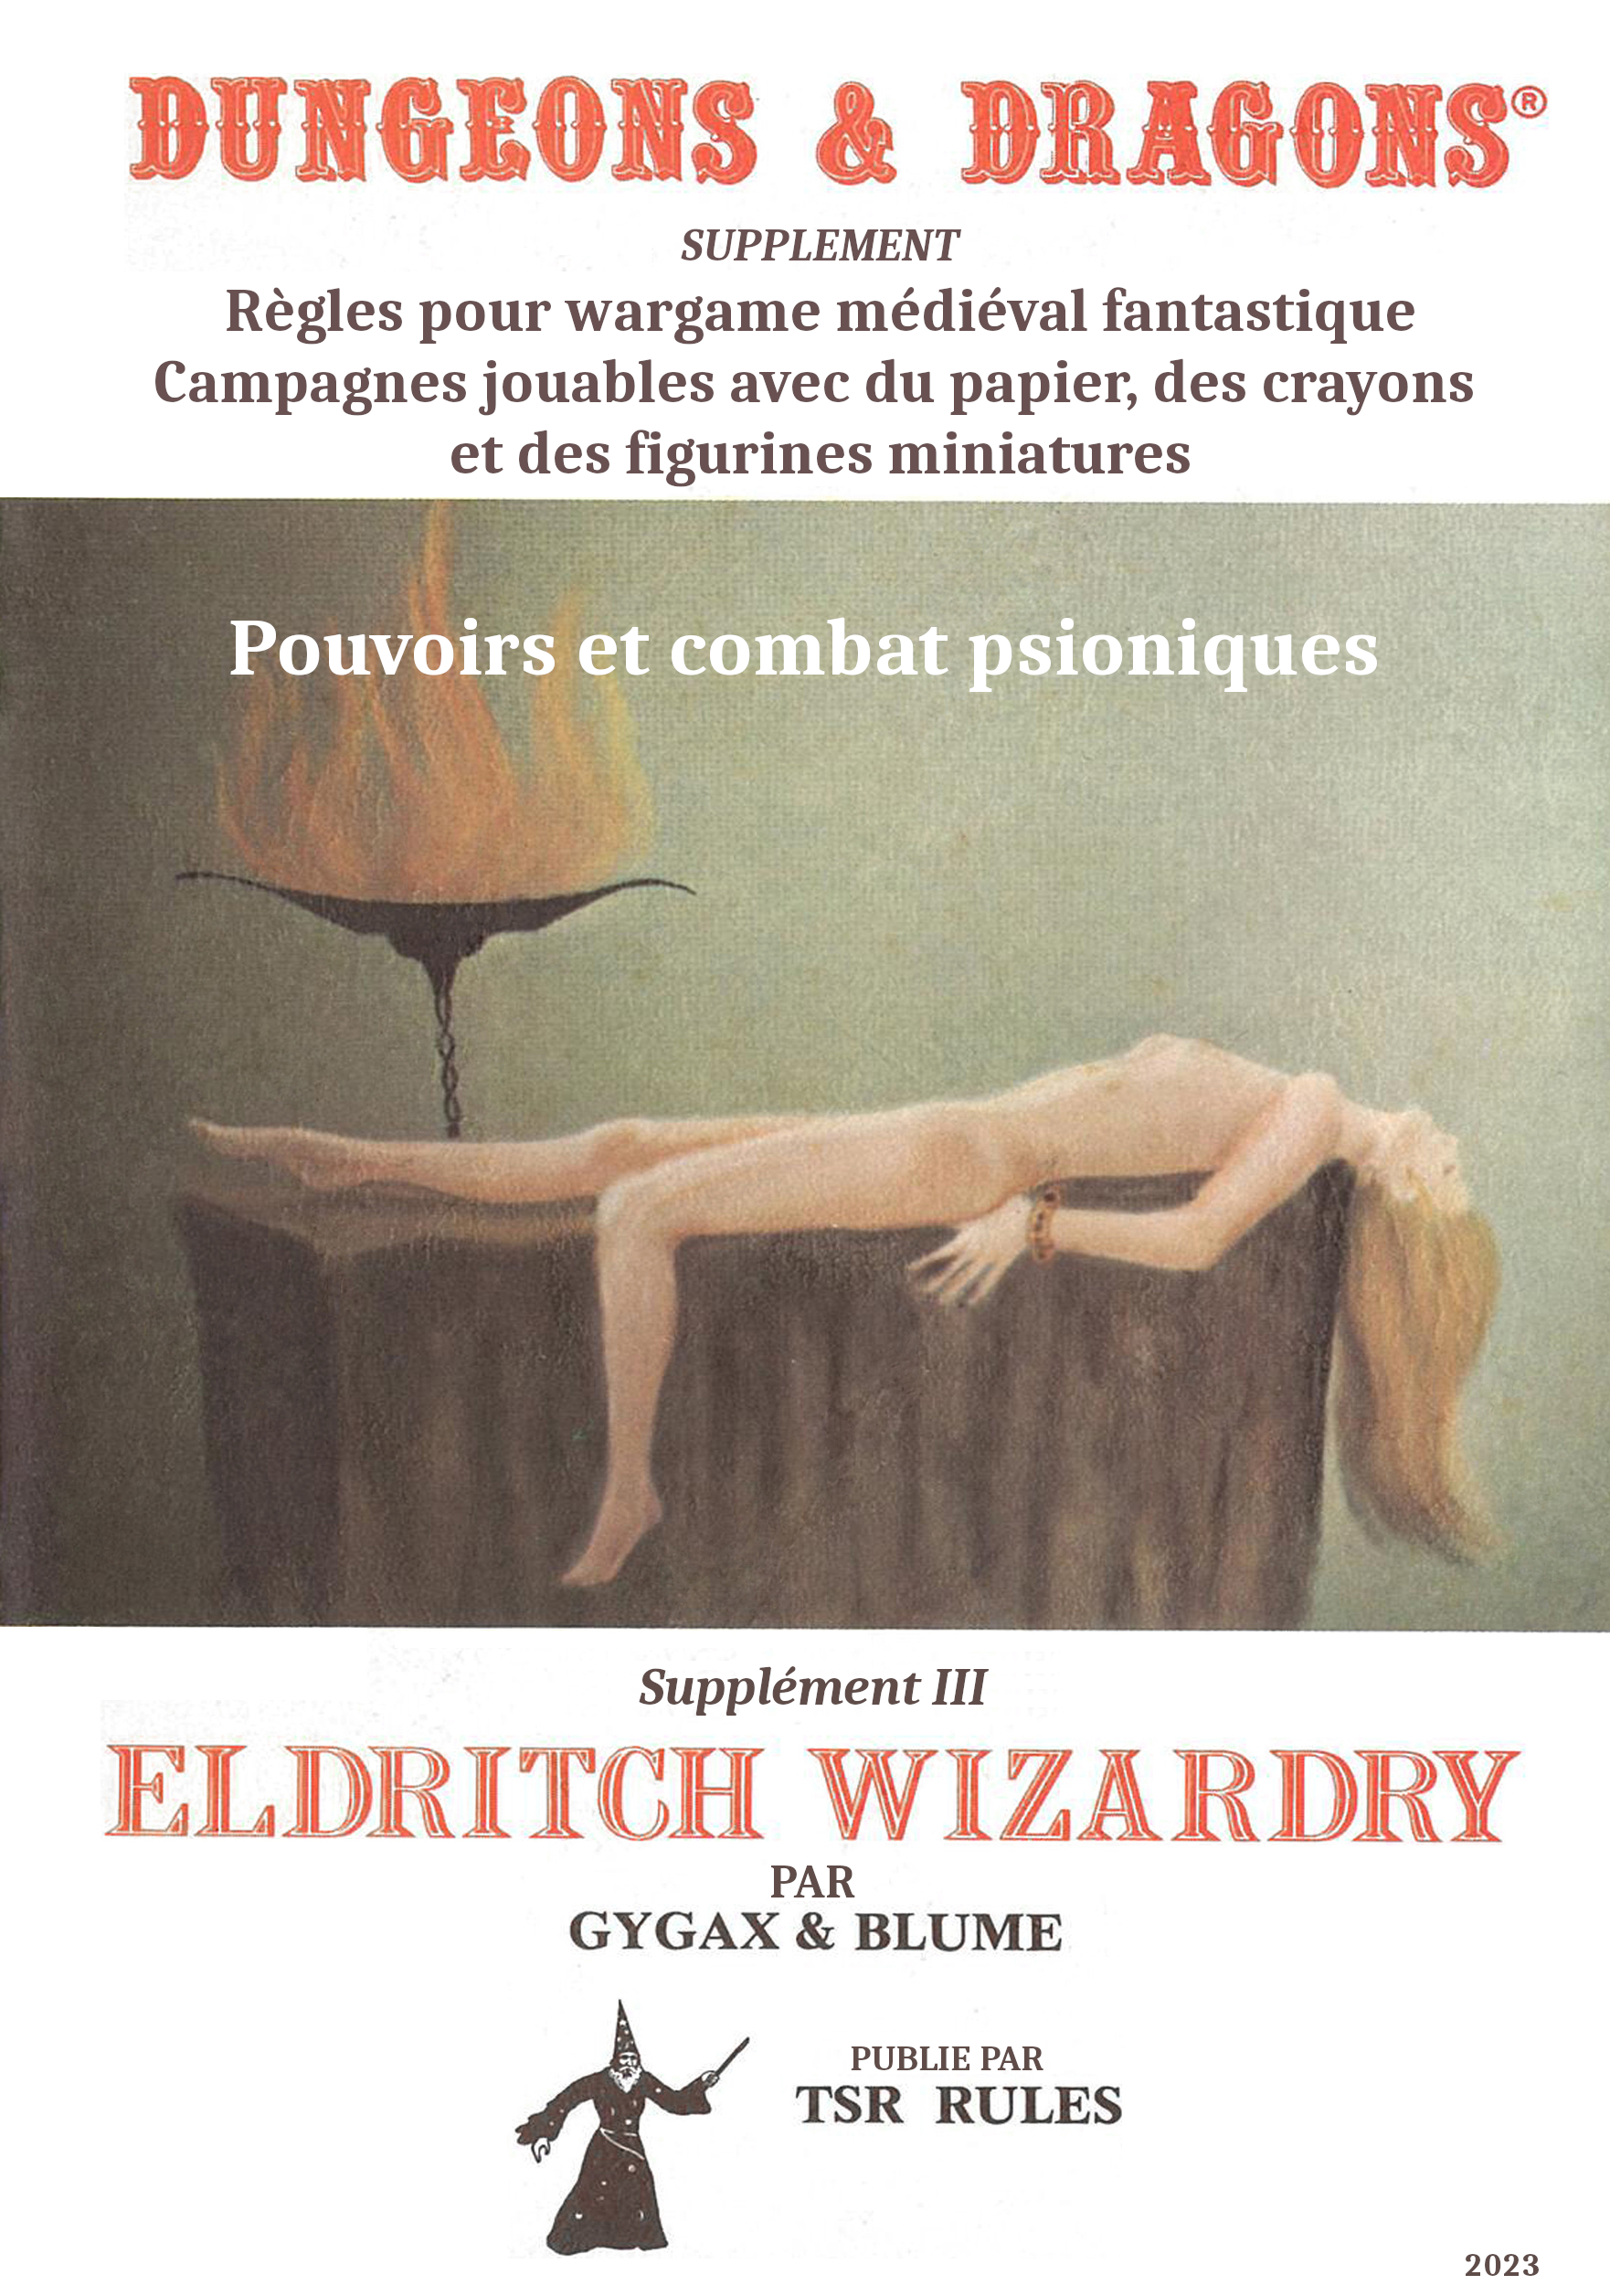
\includepdf{pagedegarde.pdf}
\newpage

{\color{white}a}

\newpage

\thispagestyle{empty}
\begin{center}
{\Huge \ODDtitlefont{DONJONS \& DRAGONS}}{\normalsize \textsuperscript{\sffamily\textregistered}}

\vspace{1.8cm}

{\Large \textbf{Supplément III}}

\vspace{1.3cm}

{\Huge \ODDtitlebisfont{ELDRITCH}}

\vspace{0.3cm}

{\Huge \ODDtitlebisfont{WIZARDRY}}

\vspace{2.0cm}

{\Large \textbf{MAGIE ANCIENNE ET PUISSANTE}}

\vspace{0.8cm}

{\large PAR}

\vspace{0.1cm}

{\large GARY GYGAX \& BRIAN BLUME}

\vspace{3cm}

Remerciements spéciaux à l'aîné Steve Marsh, Dennis Sustare (le Super Druide),

Jim Ward \& Tim Kask pour leurs suggestions et contributions !

\vspace{0.8cm}

Illustrations de Dave Sutherland, Tracy Lesch \& Gary Kwapisz

Couverture par Deborah Larson

\vspace{1cm}

{\small \textbf{\ODDtimes{2023}}}

\vspace{0.5cm}

{\small \ODDtimes{\textbf{\textcopyright\ 1976 - TSR GAMES}

\textbf{9\textsuperscript{ème} impression, novembre 1979}

\textbf{Imprimé aux U.S.A}}}
\end{center}

\vfill

{\small \noindent LES QUESTIONS SUR LES REGLES DOIVENT ETRE ACCOMPAGNEES D'UNE ENVELOPPE TIMBREE A L'ADRESSE DE L'EXPEDITEUR ET ENVOYEES A TACTICAL STUDIES RULES, POB 756, LAKE GENEVA, WISCONSIN 53247}


\newpage
%====================================================
{\color{white}a}

\vfill

\noindent {\scriptsize \textit{Ce fascicule est une adaptation par Rouboudou (https://rouboudou.itch.io) de la partie pouvoirs psioniques du livret original. Cette adaptation est une œuvre de fan, gratuite et ne pouvant être vendue.}}

\newpage

\section*{Préface}

Le livre que vous tenez maintenant dans vos mains présente de nouvelles dimensions à un système de jeu déjà fascinant. Il s'agit du troisième supplément à DONJONS \& DRAGONS, produit comme conséquence à une demande toujours croissante de nouveau matériel.

Ce livre présente aussi une nouvelle mode dans l'art subtil d'être Maître de Donjon. Fidèle à sa conception d'origine, D\&D n'était limité dans son périmètre que par l'imagination et la dévotion des Maîtres de Donjons où qu'ils soient. Les suppléments ont répondu au besoin d'idées nouvelles et de mécanismes de simulation additionnels. Mais progressivement, D\&D a perdu un peu de sa saveur, et a commencé à devenir prévisible. Cela était dû à la prolifération d'ensembles de règles ; alors que c'était très bien pour nous en tant de compagnie, c'était compliqué pour le MD. Quand tous les joueurs avaient toutes les règles en face d'eux, il devenait presque qu'impossible de les séduire à affronter le danger ou les pièges.

Le nouveau concept innovant présenté dans ces pages devrait faire long feu en réintroduisant un peu de mystère, d'incertitude et de danger, qui refont de D\&D le défi sans équivalent qu'il a toujours été. La légende retrouve sa magie inestimable originale. On ne verra plus d'aventurier imprudent descendre dans un donjon , trouver quelque chose et savoir immédiatement ce que cela fait et comment cela fonctionne. De même, les joueurs ne pourront plus envoyer un de leurs infortunés serviteurs à une mort précoce en le forçant à expérimenter à sa place.

L'introduction du combat psionique est destiné à revivifier des parties devenues stagnantes. Il ouvre de nouvelles possibilités à la fois aux joueurs et au MD, tout en intégrant un des sujets favoris des auteurs de science-fiction et de fantastique : les pouvoirs inconnus de l'esprit.

Comme pour les deux précédents suppléments, le matériel contenu dans ce livret propose le même format que les trois livrets originaux de D\&D. Les corrections et les ajouts sont indiqués dans le texte de sorte qu'ils puissent être intégrés facilement dans les règles originales.

Comme vous pourrez le noter sur la page de titre, ce supplément est le fruit de plusieurs contributeurs. Telle est la nature de la chose que vous tenez entre vos mains. D\&D a été conçu pour être un jeu libre, lié aux règles de manière souple. Nous pensons que ELDRITCH WIZARDRY favorise les principes originaux de danger, d'excitation et d'incertitude. Que vous réussissiez toujours vos jets de sauvegarde.

\vspace{1cm}

\noindent Timothy J. Kask

\noindent TSR Publications Editor

\noindent Lake Geneva, Wisconsin

\noindent 23 avril 1976

\newpage

\section*{Introduction}

Le terme anglais \texttt{psionic} a été utilisé la première fois en 1951 dans une nouvelle de science-fiction écrite par Jack Williamson, \texttt{The Greatest Invention}, publié dans le magazine \texttt{Astounding Science Fiction}. Il est la compression de deux deux termes, \texttt{psi} dans le sens de phénomène psychique et \texttt{electronics}. \texttt{Psionics} devient un terme décrivant la discipline qui étudie les phénomènes psychiques avec les moyens de l'ingénierie moderne de l'époque, soit l'électronique. Malgré la promotion de personnes comme John W. Campbell, le terme restera utilisé uniquement dans le monde de la science-fiction, avant d'être intégré dans le monde des jeux de rôles.

La version originale de Donjons \& Dragons, dite OD\&D, est publié en 1974 sous la forme de trois livrets à la couverture marron. On trouve dans le second livret, \texttt{Monstres et Trésors}, traduit en français par Porphyre et disponible sur le site de \texttt{La Forge de Papier}(la-forge-de-papier.over-blog.com), on trouve les premières références à des pouvoirs psychiques, dans le chapitre sur les épées magiques. A l'époque, le terme \texttt{psionic} n'est pas utilisé.

Ensuite, en 1976, dans le deuxième supplément \texttt{Eldritch Wizardry} cosigné par Gary Gygax et Brian Blume, les pouvoirs psychiques arrivent dans le monde des PJs et des PNJs. Les règles sont présentée de manière assez chaotique, ce qui générera vite la réputation d'un système injouable dans le monde des joueurs. Derrière la juste critique sur la présentation, beaucoup de joueurs semblent avoir rejeté le supplément en raison du fait même de proposer en extension à un jeu médiéval-fantastique des règles plus proches de la science-fiction.

Nous proposons ici une nouvelle présentation des règles psioniques du supplément \texttt{Eldritch Wizardry}. Les règles présentées sont exhaustives, précisées et réorganisées. La consultation de certains sites en américain a été nécessaire pour s'assurer de la bonne compréhension de certaines règles ambiguës qui, encore aujourd'hui, provoquent des commentaires et des incompréhensions.

Une fois éclairci, le système se montre très intéressant, non seulement parce qu'il est très "gygaxien" (on le voit notamment au travers de l'utilisation de règles gigognes), mais aussi parce qu'il est le premier système complet de psioniques proposant une façon nouvelle de voir les pouvoirs, très différente de la magie de OD\&D, façon qui inspirera beaucoup d'autres systèmes de pouvoirs dont l'utilisation est basée sur la consommation de points.

\vspace{1cm}

\noindent Rouboudou

\noindent https://orey.github.io/blog

\noindent Juillet 2023

\newpage

\section*{Index}

\newpage

\section*{Hommes \& Magie}


\newpage

\section*{Monstres \& Trésors}

\subsection*{ÉPÉES}
{\parindent0pt

Parmi les armes magiques, seules les épées possèdent certains attributs humains (et surhumains) ;
les épées ont un alignement (Loyal, Neutre ou Chaotique), un facteur d’\myunderline{intelligence}, et un score d’\myunderline{Ego} (ainsi que la détermination optionnelle de leur origine/finalité). Ces déterminations sont faites de la manière suivante :

\bigskip

\textbf{Alignement} : lancez un dé de pourcentage pour déterminer l’alignement.

\bigskip

{\parindent2.5cm
\begin{tabular}{p{2.8cm}l}
01 - 65
& L’épée est loyale \\
66 - 90
& L’épée est neutre \\
91 - 00
& L’épée est chaotique \\
\end{tabular}}

\medskip

Notons que les pourcentages ci-dessus sont inversés pour les épées ayant des capacités de drainage de
l’énergie vitale (83 sur la Table des Épées\footnote{Se référer au manuel \texttt{Eldritch Wizardry} original dans la section des objets magiques (NdT).}). Si l’épée est Chaotique, elle affecte les créatures notées entre parenthèses (clercs, pégases,
hippogriffes, ents) au lieu de ceux indiqués en premier (trolls, morts-vivants).

\medskip

Si un personnage se saisit d’une épée qui n’est pas du même alignement, il subit les dégâts suivants :

\medskip

Loi - Chaos : 2 Dés (2-12 points)

Neutralité - Loi/Chaos : 1 Dé (1-6 Points)

\medskip

Si un PNJ se voit ordonner de prendre une épée, les dégâts ne seront que la moitié de ceux indiqués ci-dessus, le personnage n’agissant pas de son propre chef. De plus, l’épée pourrait libérer celui qui l’a ramassée
d’un sortilège, le faire changer d’alignement, ou lui faire gagner des pouvoirs qui le feraient échapper au
contrôle de son précédent maître.

\medskip

De plus, si l‘Intelligence/Égoïsme (voir ci-dessous) de l’épée est supérieur de 6 points ou plus que celle de
celui/celle qui la prend, l’épée contrôlera le personnage, lui faisant prendre le même alignement et agir en
conséquence immédiatement. Cela voudrait dire, par exemple, que le servant d’un personnage Loyal à qui
l’on ordonnerait de prendre une épée Neutre, et qui serait possédé par cette dernière, pourrait délibérément
mentir sur ses pouvoirs, tandis que, dans le cas d’une épée chaotique, il attaquerait !

\medskip

Après avoir déterminé l’alignement, c’est à l’intelligence de l’épée d’être lancée.

\medskip

\myunderline{Intelligence} : deux facteurs dépendent de l’Intelligence : les pouvoirs mentaux et l’aptitude à communiquer.
Tous deux sont déterminés par le même jet de dé.

\medskip

\begin{tabular}{p{2.5cm} l p{2cm}}
Intelligence & &\myunderline{Capacités de} \\
(\myunderline{Dé}) & \myunderline{Pouvoirs mentaux} & \myunderline{communication} \\
1-6
& Aucun & Aucune* \\
7
& Un pouvoir primaire & Empathie \\
8
& Deux pouvoirs primaires & Empathie \\
9
& Trois pouvoirs primaires & Empathie \\
10
& Trois pouvoirs primaires et l’usage de langues** & Parole \\
11
& Comme 10 ci-dessus et aussi Lecture de la magie & Parole \\
12
& Comme 11 ci-dessus et aussi un pouvoir extraordinaire & Télépathie \\
\end{tabular}

\medskip

* Même incapable de communiquer, l’épée confère au porteur ses pouvoirs, mais ceux-ci devront être découverts par l’utilisateur.

** Le nombre de langues parlées en \myunderline{plus de la langue d’alignement de l’épée} est déterminé par un jet de dé :

\medskip

\myunderline{Table des Pouvoirs primaires}


Dé
01-15
16-30
31-40
41-50
51-60
61-70
71-80
81-90
91-95
96-99
00
28
Pouvoir
Détection des parois \& salles coulissantes
Détection des passages inclinés
Détection des portes secrètes
Détection des pièges
Détecter l'invisible
Détection du mal ou de l'or
Détection du métal \& de quelle sorte
Détection de la magie
Détection des gemmes
Relancer deux fois, ignorer les scores supérieurs à 95
sauf 00
Lancer un jet sur la table des pouvoirs extraordinaires
Dé
01-50
51-70
71-85
86-90
90-99
00
\# langues parlées
Un
Deux
Trois
Quatre
Cinq
Lancer deux fois,
ignorer les 00


Table des Pouvoirs extraordinaires
Dé
01-10
11-20
21-30
31-40
41-50
51-59
60-68
69-77
78-82
83-87
88-92
93-97
98-99
00
Capacités
Clairaudience
Clairvoyance
ESP
Télépathie
Télékinésie
Téléportation
Vision rayon X
Génération d'illusion
Lévitation
Vol
Soins (1point/6 tours ou 6 points/jr)
1-4 fois la force normale pendant 1-10 jours, une fois par jour
Relancer deux fois, ignorer les jets au-dessus de 97
Relancer trois fois, ignorer les jets au-dessus de 97
Tous les pouvoirs primaires et pouvoirs extraordinaires sont transmis à l’utilisateur de l’épée. Si la même
capacité est tirée deux fois aux dés, cela indique qu’elle est au double de la normale en termes de force,
portée, exactitude, etc.
Ego : seules les épées avec une Intelligence de 7 ou plus ont un score d’Égo. L’Égo va de 1 à 12. L’Ego de
l’épée peut provoquer les choses suivantes :
1. Obliger l’utilisateur à se défaire d’autres meilleures armes.
2. Conduire l’utilisateur dans des situations dangereuses afin d’exalter ses prouesses au combat
3. Se laisser capturer par un personnage/une créature de niveau plus élevé, considéré plus digne du
pouvoir de l’épée
4. Se rendre à une créature/un personnage de niveau inférieur pour pouvoir plus facilement contrô-
ler son utilisateur
5. Exiger qu’une partie des trésors conquis soit consacrée à l’achat d’un fourreau de qualité, d’in-
crustations de pierreries ou en protections magiques.
Lorsque survient une situation où existe l‘une des possibilités décrites ci-dessus, l’Ego de l’épée rentre en
jeu. Celui-ci s’exercera tout au long de sa relation avec son utilisateur, bien qu’une vraie relation puisse
se mettre en place si l’alignement et les objectifs du personnage-joueur coïncide avec les origines / les
objectifs de l’épée.
Déterminer chacun comme suit :
Influence de l’Ego dans des situations critiques. L’arbitre additionne l’Intelligence et l’Ego de l’épée
(résultat de 8 à 24), et ajoute un point supplémentaire pour chaque pouvoir extraordinaire (de 1
à 4). Ce total (allant de 8 à 28) est comparé au total de la force et intelligence du personnage,
éventuellement modifié en fonction de l’état de santé de ce dernier. Si le personnage est reposé et
relativement indemne de tout dommage (moins de 10 % de dégâts) de 1-6 points sont ajoutés à
ce total (de 7-42).
S’il est fatigué mentalement ou physiquement, ou si les dégâts subis sont entre 10 % et 50 %, de

1 – 4 points sont soustraits à ce total (de 2 – 35). Si les dégâts subis sont au-dessus de 50 %, ou
si le personnage est soumis à une sérieuse tension mentale par quelque forme de magie de 2 – 8
points sont soustraits à ce total (de 0 -34).
Différence
6 ou plus
2 à 5
0 à 1
Résultat
Le score le plus élevé l’emporte
75 % de chances que le score le plus élevé l’emporte
50 % pour chaque cas
Influence de l’Ego dans les relations au long cours avec l’utilisateur. Cette détermination est très
simple, il s’agit juste de comparer le score d’Ego de l’épée (1–12) avec le niveau du combattant
qui l’utilise. Consulter la table des situations critiques ci-dessus. Si l’une ou l’autre partie a une
différence de 6 ou plus, la partie en question prévaut toujours, et aucun autre jet (y compris dans
les situations critiques) ne sera nécessaire. Une différence positive de 2–5 indique que la partie
avec le score le plus élevé l’emporte généralement, et les jets n’auront à être faits que dans les si-
tuations critiques. Une différence de 0-1 indique qu’une lutte permanente existe entre l’épée et son
utilisateur, et en cas de situation critique, chacun devra faire un jet pour savoir lequel l’emporte.
Origines et objectifs : chaque épée est certes d’origine loyale, neutre ou chaotique, mais certaines armes
ont été forgées par des puissances supérieures dans un but précis. Déterminez par un jet de pourcentage si
une épée à une telle raison d’être : un résultat de 91 ou plus indique que l’épée est investie d’une mission
spécifique. Les épées ayant un objectif précis voient leur Intelligence et Ego automatiquement portés au score
maximum, et gagnent un pouvoir spécial :
Loi : pouvoir de paralyser les adversaires chaotiques.
Neutralité : bonus de +1 aux jets de sauvegarde.
Chaos : pouvoir de désintégrer les adversaires loyaux.
Ces pouvoirs spéciaux ne s’exercent que contre ceux que l’épée a pour mission de détruire, ou bien ceux qui
servent de telle créature.
Objectifs :
Tuer les magiciens
Tuer des clercs
Tuer des combattants
Tuer des monstres
Défaire la Loi
Défaire le Chaos
De cette façon, une épée habitée par la Loi dans le but de tuer des magiciens (chaotiques) paralysera ces person-
nages magiques ainsi que leurs séides, mais n’utilisera pas ses pouvoirs de paralysie contre un géant de passage.
Les épées ayant des objectifs d’ordre général, par contre, utiliseront leurs pouvoirs pour triompher de tout ennemi
de nature loyale/chaotique. Les épées neutres avec un objectif spécial agissent de la même façon, que ce soit
contre la Loi ou le Chaos.
Les épées ayant un objectif désigné seront toujours toutes à leur tâche, et toute tentative par leur utilisateur d’aller
à leur encontre provoquera immédiatement un jet d’influence.
BONUS AUX DÉGÂTS DES ÉPÉES. Les épées ont toutes un bonus en ce qui concerne la probabilité de toucher un
adversaire, mais certaines ont également un bonus aux points de dégâts qu’elles infligent quand elles touchent. Ce
sont les épées +2 ou +3 contre une créature spécifique, mais non celles qui ont un bonus générique de +2 ou +3.

}% parindent

\begin{verbatim}
---
tags:
    - Ambre
    - D&D
    - Zelazni
---

# Vocabulaire

Alors que l'on dit plutôt en français, "pouvoirs psychiques", le terme américain "psionic" est entré progressivement dans le vocabulaire des jeux de rôles, souvent en étant francisé en "psionique". Dans cet article, nous nous limiterons à l'usage du terme "psychique" en français, le terme "psionic" étant réservé à la citation d'ouvrages en anglais.

# 1976 - OD&D au début de tout (comme souvent)

## Introduction

![Alt text](../images/eldritch-wizardry.png)

En 1976 sort le livre VI de *Dungeons & Dragons* avec le titre *Eldritch Wizardry* cosigné de [Gary Gygax](https://github.com/orey/DandD/tree/master/GaryGygax) et de Brain Blume. Ce livre d'une soixantaine de pages contient essentiellement des suppléments sur les pouvoirs psychiques, sur le druide en tant que classe de personnage et sur les démons.

Ledit supplément est disponible sur [archive.org](https://archive.org/details/tsr02005supplement3eldritchwizardy). Il n'a pas été traduit en français à ma connaissance alors que les règles de OD&D l'ont été : voir sur le très bon site [La Forge de papier](http://la-forge-de-papier.over-blog.com/2017/09/donjons-dragons-la-boite-blanche-elle-aussi-en-francais.html).

Il semble que ce soit la première apparition des pouvoirs psychiques dans le monde du JDR. Leur apparition au sein de *D&D* a quelque chose d'étrange, car on pourrait y voir une collision de diverses influences dans la fantasy: le médiéval-fantastique qui favorise la magie et les pouvoirs psychiques qui sent plus le JDR contemporain ou futuriste.

D&D propose les pouvoirs psy comme un genre de supplément optionnel pour "pimenter" les parties. L'introduction de 1976 de [Tim Kask](https://en.wikipedia.org/wiki/Tim_Kask) dudit livre est amusante :

*L'introduction du combat psionique s'attache à redynamiser des jeux devenus ternes. Cela ouvre des possibilités inédites à la fois pour les joueurs et le MD et, ce faisant, cela permet de se reconnecter à l'un des thèmes favoris des écrivains de science-fiction et de fantasy : les pouvoirs inconnus de l'esprit.*

Pour autant, en lisant entre les lignes, l'introduction des démons dans le jeu semble pousser Gygax à créer les règles des pouvoirs psychiques, mieux adaptés, selon lui, à représenter les pouvoirs de certains démons.

Comme souvent dans OD&D, les règles sont confuses, incomplètes, éclatées dans le tout le livret, entrecoupées de choses qui n'ont rien à voir (le Druide, un système de combat alternatif basé sur la **Dextérité Ajustée**, etc.). Au niveau édition, *Eldritch Wizardry* est un des pires exemples de l'époque.

## Obtention des Pouvoirs Psychiques (PoP)

A la création du PJ, un score de 15 ou plus dans INTelligence, WISdom ou CHArisma donne la possibilité de tester si le personnage dispose d'un pouvoir psy (si le personnage est humain). Il est nécessaire de faire 91 ou plus sur 1d100 pour que ce soit le cas. Les moines et les druides ne peuvent pas avoir de pouvoirs psychiques.

Si le personnage est éligible, il faut faire un nouveau jet de 1d100 pour déterminer le **potentiel psychique** (PP, purement aléatoire). Suivant le PP, le PJ obtient un malus ou un bonus pour avoir des **pouvoirs psychiques** (PoP, de -6% à +3%).

| PP (1d100) | Bonus/Malus au jet d'obtention de PoP (BMPoP) |
|------------|-----------------------------------------------|
| 01–10      | -6% par niveau (cumulatif)                    |
| 11–25      | -5% par niveau (cumulatif)                    |
| 26–50      | -4% par niveau (cumulatif)                    |
| 51–75      | Aucun                                         |
| 76–90      | +1% par niveau (cumulatif)                    |
| 91–99      | +2% par niveau (cumulatif)                    |
| 00         | +3% par niveau (cumulatif)                    |

La chance de base pour avoir un PoP est de 10% + BMPoP par niveau. Ainsi, un perso du 4ème niveau avec un PP de 90 aura une base de 10 + 1 = 11 soit 11 x 4 = 44% de chances d'avoir un PoP. Cela veut dire aussi qu'un personnage de niveau 10 aura 100% d'avoir un PoP.

Notons enfin que donc, ce jet se produit à chaque changement de niveau.

Cerise sur le gâteau : si le PJ obtient un PoP, alors s'il réussit un jet de 1d100 sous son PP, il en a automatiquement un second !

Nous sommes en plein dans le monde Gygaxien des **règles gigognes** :

* R1 : INT ou WIS ou CHA > 15,
* R2 : Si R1 OK, jet de 1d100 pour PP et BMPoP,
* R3 : Quand R2 OK, jet de BMPoP pour obtenir un PoP,
* R4 : Si R3 OK, si succès, alors jet de PP pour obtenir un second PoP.

Nous verrons apparaître ce genre de règles gigognes dans les autres éditions de D&D signées de Gygax.

## Pouvoirs psychiques (PoP)

### Liste des pouvoirs

La liste originale est présentée ci-dessous.

![Listedescompetencespsioniques](../images/od&d-psionics.png)

La liste des PoP est fournie ci-dessous, retriée par type (interprétation personnelle) et par classe de personnages.

| Pouvoir Psychique (PoP)           | Type | Guerriers & Voleurs | Magiciens  | Clercs     |
|-----------------------------------|------|---------------------|------------|------------|
| Réduction                         | A    | 1 Oui (B)           | 1 Oui (B)  |            |
| Expansion                         | A    | 2 Oui (B)           | 2 Oui (B)  |            |
| Lévitation                        | A    | 3 Oui (B)           | 3 Oui (B)  | 1 Oui (B)  |
| Changer le poids du corps         | A    | 4 Oui (B)           |            | 2 Oui (B)  |
| Corps comme arme                  | A    | 5 Oui (B)           |            |            |
| Réarrangement moléculaire         | A    | 6 Oui (S)           |            | 3 Oui (S)  |
| Manipulation moléculaire          | A    | 7 Oui (S)           |            |            |
| Contrôle du corps                 | A    | 8 Oui (S)           |            |            |
| Barrière mentale                  | A    | 9 Oui (S)           |            |            |
| Agitation moléculaire             | A    |                     | 4 Oui (B)  |            |
| Altération de la forme            | A    |                     | 5 Oui (S)  |            |
| Contrôle cellulaire               | A    |                     |            | 4 Oui (B)  |
| Contrôle de l'esprit sur le corps | A    | 10 Oui (B)          |            | 5 Oui (B)  |
| Invisibilité                      | A    | 11 Oui (B)          |            |            |
| Hibernation                       | A    | 12 Oui (B)          |            |            |
| Télékinésie                       | A    | 13 Oui (S)          | 6 Oui (S)  |            |
| Contrôle de l'énergie             | A    | 14 Oui (S)          |            |            |
| Domination                        | B    | 15 Oui (B)          |            | 6 Oui (B)  |
| Hypnose                           | B    |                     | 7 Oui (B)  | 7 Oui (B)  |
| Projection télépathique           | B    |                     | 8 Oui (S)  | 8 Oui (S)  |
| Altération de l'aura              | B    |                     |            | 9 Oui (S)  |
| Domination des masses             | B    |                     |            | 10 Oui (S) |
| ESP                               | B    |                     | 9 Oui (B)  | 11 Oui (B) |
| Empathie                          | B    |                     |            | 12 Oui (S) |
| Télépathie animale                | B    |                     |            | 13 Oui (B) |
| Prémonition                       | C    | 16 Oui (B)          | 10 Oui (S) | 14 Oui (S) |
| Clairaudience                     | C    | 17 Oui (B)          | 11 Oui (B) |            |
| Clairvoyance                      | C    | 18 Oui (B)          | 12 Oui (B) |            |
| Détection du mal/du bien          | C    |                     | 13 Oui (B) | 15 Oui (B) |
| Détection de la magie             | C    |                     | 14 Oui (B) |            |
| Marche dimensionnelle             | D    | 19 Oui (S)          |            | 16 Oui (S) |
| Projection astrale                | D    | 20 Oui (S)          | 15 Oui (S) | 17 Oui (S) |
| Porte dimensionnelle              | D    |                     | 16 Oui (S) |            |
| Téléportation                     | D    |                     | 17 Oui (S) |            |
| Substance éthérée                 | D    |                     | 18 Oui (S) |            |
| Voyage probabiliste               | D    |                     |            | 18 Oui (S) |

Nous pouvons classer ces pouvoirs en plusieurs catégories (ce n'est pas dans le livre original) :

* A : Contrôle de la matière au niveau moléculaire, voire atomique,
* B : Contrôle via l'esprit de l'esprit,
* C : Sens,
* D : Voyage psychique.

Les pouvoirs sont présents chez les types de personnages soient au niveau Basique (B) soit au niveau Supérieur (S). Le fait qu'un PoP soit Supérieur ne se traduit (dans les règles) que par le fait qu'elle soit détectable par un autre personnage ayant des pouvoirs psy au double de la portée du pouvoir (voir plus bas détection des pouvoirs psychiques).

Les PJ ne peuvent pas avoir plus de PoP Supérieurs que de PoP Basiques.

Cette distinction est peu développée et on imagine que le but était d'avoir la possibilité de deux puissances différentes dans les mêmes pouvoirs. Par contre, les pouvoirs eux-mêmes n'utilisent pas cette distinction.

La détermination des PoPs est aléatoire mais il est suggéré de restreindre le choix à des types de PoP cohérents.

### A - Contrôle de la matière et de l'énergie

On retrouve dans cette dimension pas mal de pouvoirs :

* Réduction ;
* Expansion ;
* Lévitation, qui est un moyen de changer le poids du corps ;
* Changer le poids du corps (*Body Equilibrium*), notamment pour marcher sur l'eau ;
* Corps comme arme (*Body Weaponry*) ;
* Réarrangement moléculaire, qui transforme les métaux ;
* Manipulation moléculaire, qui permet de rendre fragile différentes matières dures ;
* Contrôle du corps, qui permet d'adapter le corps à des conditions extrêmes comme le froid extrême, le feu, les fumées empoisonnées, etc. ;
* Barrière mentale ;
* Agitation moléculaire, agit un peu comme un four à micro-ondes ;
* Altération de la forme, pour se changer en quelqu'un d'autre ;
* Contrôle de l'esprit sur le corps, pour se passer de manger, de boire et de dormir ;
* Invisibilité ;
* Hibernation (*Suspend Animation*), ou comment suspendre ses fonctions vitales ;
* Télékinésie, contrôle du mouvement des objets par la pensée ;
* Contrôle de l'énergie, ou comment dissiper des énergies agressives ;
* Contrôle cellulaire (*Cellular Adjustment*), qui permet de soigner les blessures et les maladies.

### B - Contrôle via l'esprit de l'esprit

On retrouve les pouvoirs suivants :

* Domination, pour forcer une personne à faire ce que le PJ souhaite ;
* Hypnose, contrôle des esprits faibles ;
* Projection télépathique, envoyer des messages ou influence une personne ;
* Altération de l'aura ;
* Domination des masses ;
* ESP ;
* Empathie ;
* Télépathie animale.

### C - Sens

On retrouve les pouvoirs suivants :

* Prémonition ;
* Clairaudience ;
* Clairvoyance ;
* Détection du mal/du bien ;
* Détection de la magie.

### D - Voyage psychique

* Marche dimensionnelle ;
* Projection astrale ;
* Porte dimensionnelle
* Téléportation
* Substance éthérée ;
* Voyage probabiliste, une projection astrale avec le corps permettant de passer à travers les plans et les mondes parallèles (comme dans la *Saga des Princes d'Ambres* de Zelazni).

## Modes d'Attaque et Modes de Défense

Une fois que le PJ a son premier PoP, il gagne son premier **Mode d'Attaque** psychique (MA) : *Explosion psionique* (voir tableau ci-dessous).

Les autres MA sont gagnés tous les 4 PoP (5 pour les Guerriers).

Cette dernière consigne est un peu vague. Elle sous-entend que, lors du passage de niveau, le PJ ayant des pouvoirs psychiques va refaire un test pour avoir un nouveau PoP (sachant qu'il peut en obtenir au maximum deux par niveau). Il gagnera un mode d'attaque alors en fonction du nombre de PoP dont il dispose.

Concernant les **Modes de Défense** (MD), encore une fois les règles ne sont pas claires. Il est dit qu'ils sont acquis à raison de un tous les 3 PoP acquis (4 pour les Guerriers).

Comme les PJs ayant des pouvoirs psychiques sont capables de combattre psychiquement, il faut supposer que les MDs marchent comme pour les MAs et que le PJ gagne son premier MD avec son premier PoP, puis ensuite tous les 3 (ou 4) PoP acquis.

Une autre interprétation possible serait qu'il faut vraiment avoir 3 ou 4 PoP pour gagner son premier MD. Je trouve cette interprétation un peu bizarre au regard de la suite qui présuppose, dans le combat psionique, que l'attaquant psy a un MA et que le défenseur a un MD. Un défenseur ayant des pouvoirs psychiques sans MD ouvre une brèche dans le système.

Il n'est pas expliqué comment les MA/MD sont attribués : aléatoirement (D6 en rejouant le 6) ou séquentiellement, en utilisant les lettres, ou par simple choix. Comme la puissance de ces attaques est diverse et non linéaire, je pense pas que les lettres soient très importantes pour les MA. Pour les MD, il y a une certaine progression. Au DM de choisir son mode d'attribution.

La liste des modes d'attaque et de défense est présentée ci-dessous avec leur coût en **Force Psionique** entre parenthèses.

| Modes d'Attaque (MA), toutes classes     | Modes de Défense (MD), toutes classes |
|------------------------------------------|---------------------------------------|
| A. Explosion psionique (20)[x3]          | F. Esprit vide (1)                    |
| B. Poussée de l'esprit (10)[x1]          | G. Bouclier de pensée (2)             |
| C. Coup de fouet sur l'ego (15)[x3]      | H. Barrières mentales (4)             |
| D. Imposition d'identité (10)[x1]        | I. Forteresse intellectuelle (7)      |
| E. Écrasement psychique (25&spades;)[x3] | J. Tour de volonté de fer (10)        |

&spades; Si le PJ possède moins de 25 points de FP, il est demandé au MJ de "modifier la probabilité de succès de manière *ad hoc*".

L'utilisation des MAs peut être détectée par un PJ ou PNJ ayant des pouvoirs psychiques. Le facteur entre crochets donne le multiplicateur de portée du MA dans lequel le PJ ou PNJ peut détecter son usage. Pour mémoire, les pouvoirs

## Force Psionique (FP), Force Psionique d'Attaque (FPA) et de Défense (FPD)

Les formules sont les suivantes :

* FPA = PP + 2 x nombre(PoP) + 5 x nombre(MA) + 5 x nombre(MD)
* FPD = FPA
* FP = FPA + FPD = 2 x FPA

Ces scores serviront de réservoirs de points pour les attaques et les défenses psychiques en combat psychique, mais aussi pour les divers PoP que les PJs auront accumulés et dont le coût est expliqué dans les descriptions.

A chaque fois que de la FP est consommée, il faut répartir la consommation à 50%-50% entre la FPA et la FPD, cela pour toutes les consommations. En gros, la FP est un réservoir de points divisés en deux avec une consommation égale dans les deux sous-réservoirs (cela vaut aussi pour la consommation des points en combat, soit avec les MA et MD).

La FP se récupère assez vite en cessant toute activité psychique et en suivant les indications de la table suivante.

| Activité                            | Gain en FP          |
|-------------------------------------|---------------------|
| Marcher, parler et autres activités | 6 points par heure  |
| Se reposer tranquillement           | 12 points par heure |
| Dormir                              | 24 points par heure |

## Détection des PoP et des MA

La table ci-dessous présente les règles de détection des PoP et MA (nous avons utilisé les lettres pour désigner les MA) de PJs ou PNJs ayant des pouvoirs psychiques et détectant dans leur voisinage des créatures utilisant des pouvoirs.

| Type                     | Niveau/Nom | Portée de la détection | % de base | Cumulatif par tour |
|--------------------------|------------|------------------------|-----------|--------------------|
| PoP                      | Basique    | Portée du pouvoir      | 10%       | Oui (+10%)         |
| PoP                      | Supérieur  | 2 x Portée du pouvoir  | 10%       | Oui (+10%)         |
| MA                       | A, C, E    | 3 x Portée du pouvoir  | 10%       | Oui (+10%)         |
| MA                       | B, D       | Portée du pouvoir      | 10%       | Oui (+10%)         |
| Objet psy                | -          | Portée du pouvoir      | 10%       | Oui (+10%)         |
| Sort (idem psy)          | -          | Portée du sort         | 10%       | Oui (+10%)         |
| Objet magique (idem psy) | -          | Portée du sort         | 10%       | Oui (+10%)         |

Si le pouvoir est utilisé en continu, alors les chances de détection dans le cadre de la portée de détection grandissent de 10% par tour.

La créature qui détecte ne pourra pas détecter un pouvoir qu'elle n'a pas, mais pourra, au premier tour détecter dans quelle direction le pouvoir est utilisé, et au second tour avec quelle puissance "relative" ce pouvoir est utilisé.

Les sorts qui sont similaires aux pouvoirs psychiques seront détectés de la même façon que lesdits pouvoirs. Les objets magiques qui ont les mêmes fonctions que les objets psychiques seront, eux-aussi, détectés de la même façon.

## Le PJ psionique selon OD&D

Le PJ psionique a donc les caractéristiques suivantes :

* PP avec BMPoP,
* Liste des PoPs,
* FP = FPA + FPD,
* Listes des MAs et MDs.

## Combat psychique




*En cours*

## Liens



<div class="mydate">03-20 juin 2023</div>


\end{verbatim}




\end{document}
